\begin{frame}
    \frametitle{ICECATS Podcast Timeline}

    \textbf{Alvarpi\dh{} Era:}
    \begin{itemize}
        \item Syndicated on the Icelandic podcast platform Alvarpi\dh{} on the news site N\'{u}t\'{i}minn.
        \item Debut on February 23\textsuperscript{rd} 2017 (Alvarpi\dh's 3\textsuperscript{rd} birthday).
        \item Shared the platform with other renowned podcasts like \emph{Hefnendur} and \emph{Englaryk}.
        \item Last aired on November 1\textsuperscript{st} 2018, after 46 episodes.
    \end{itemize}

    \textbf{Storytel Era:}
    \begin{itemize}
        \item Syndicated on the Icelandic audiobook platform Storytel.
        \item First of three podcasts ever featured on the platform
        (with \emph{Skr\ae{}\dh{}ur} and \emph{Seg\dh{}u m\'{e}r s\"{o}gu})
        \item Debut March 7\textsuperscript{th} 2019, and completed after
        96 episodes on December 17\textsuperscript{th}, 2020.
    \end{itemize}

\end{frame}


\begin{frame}
    \frametitle{Podcast on Alvarpi\dh{}: Listenership on \url{nutiminn.is}}
    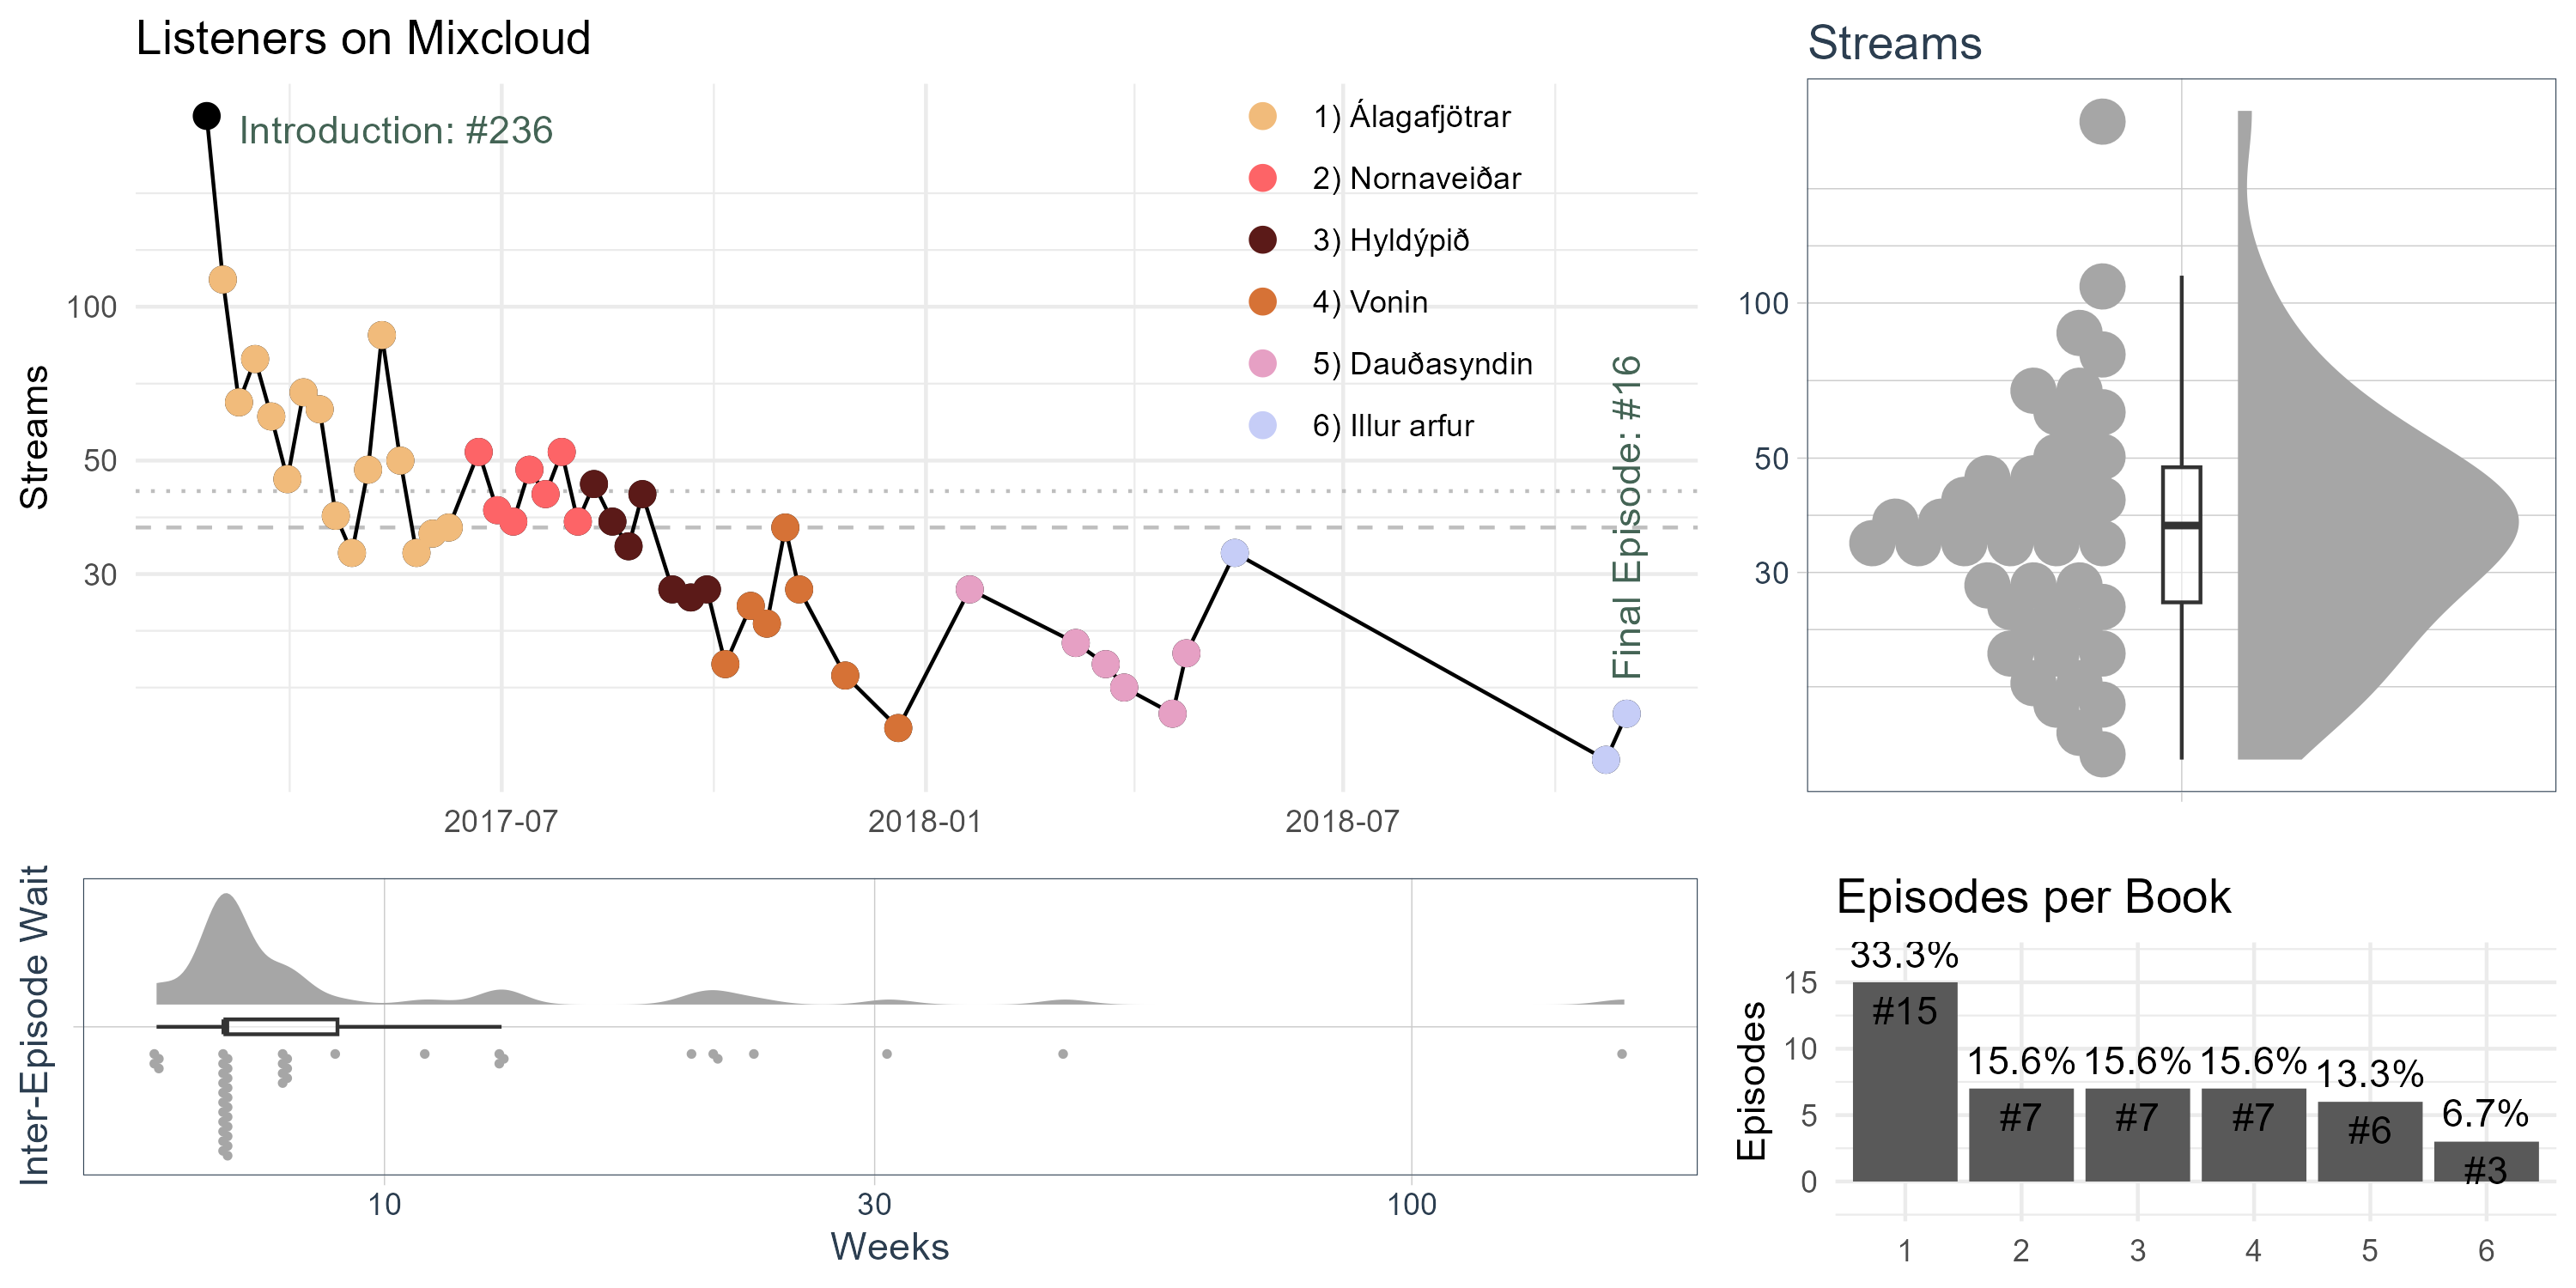
\includegraphics[width=\textwidth]{charts/alvarpid_listeners.png}

    \begin{itemize}
        \item 46 episodes, 20 months, 5.5 books
        \item 2231 minutes -- 37 hours -- 1.5 days of continuous listening
        \item Roughly 1040 streams per episode (thereof ~40 in browser)
    \end{itemize}

\end{frame}


\begin{frame}
    \frametitle{Podcast on Storytel: Hours Rambled}
    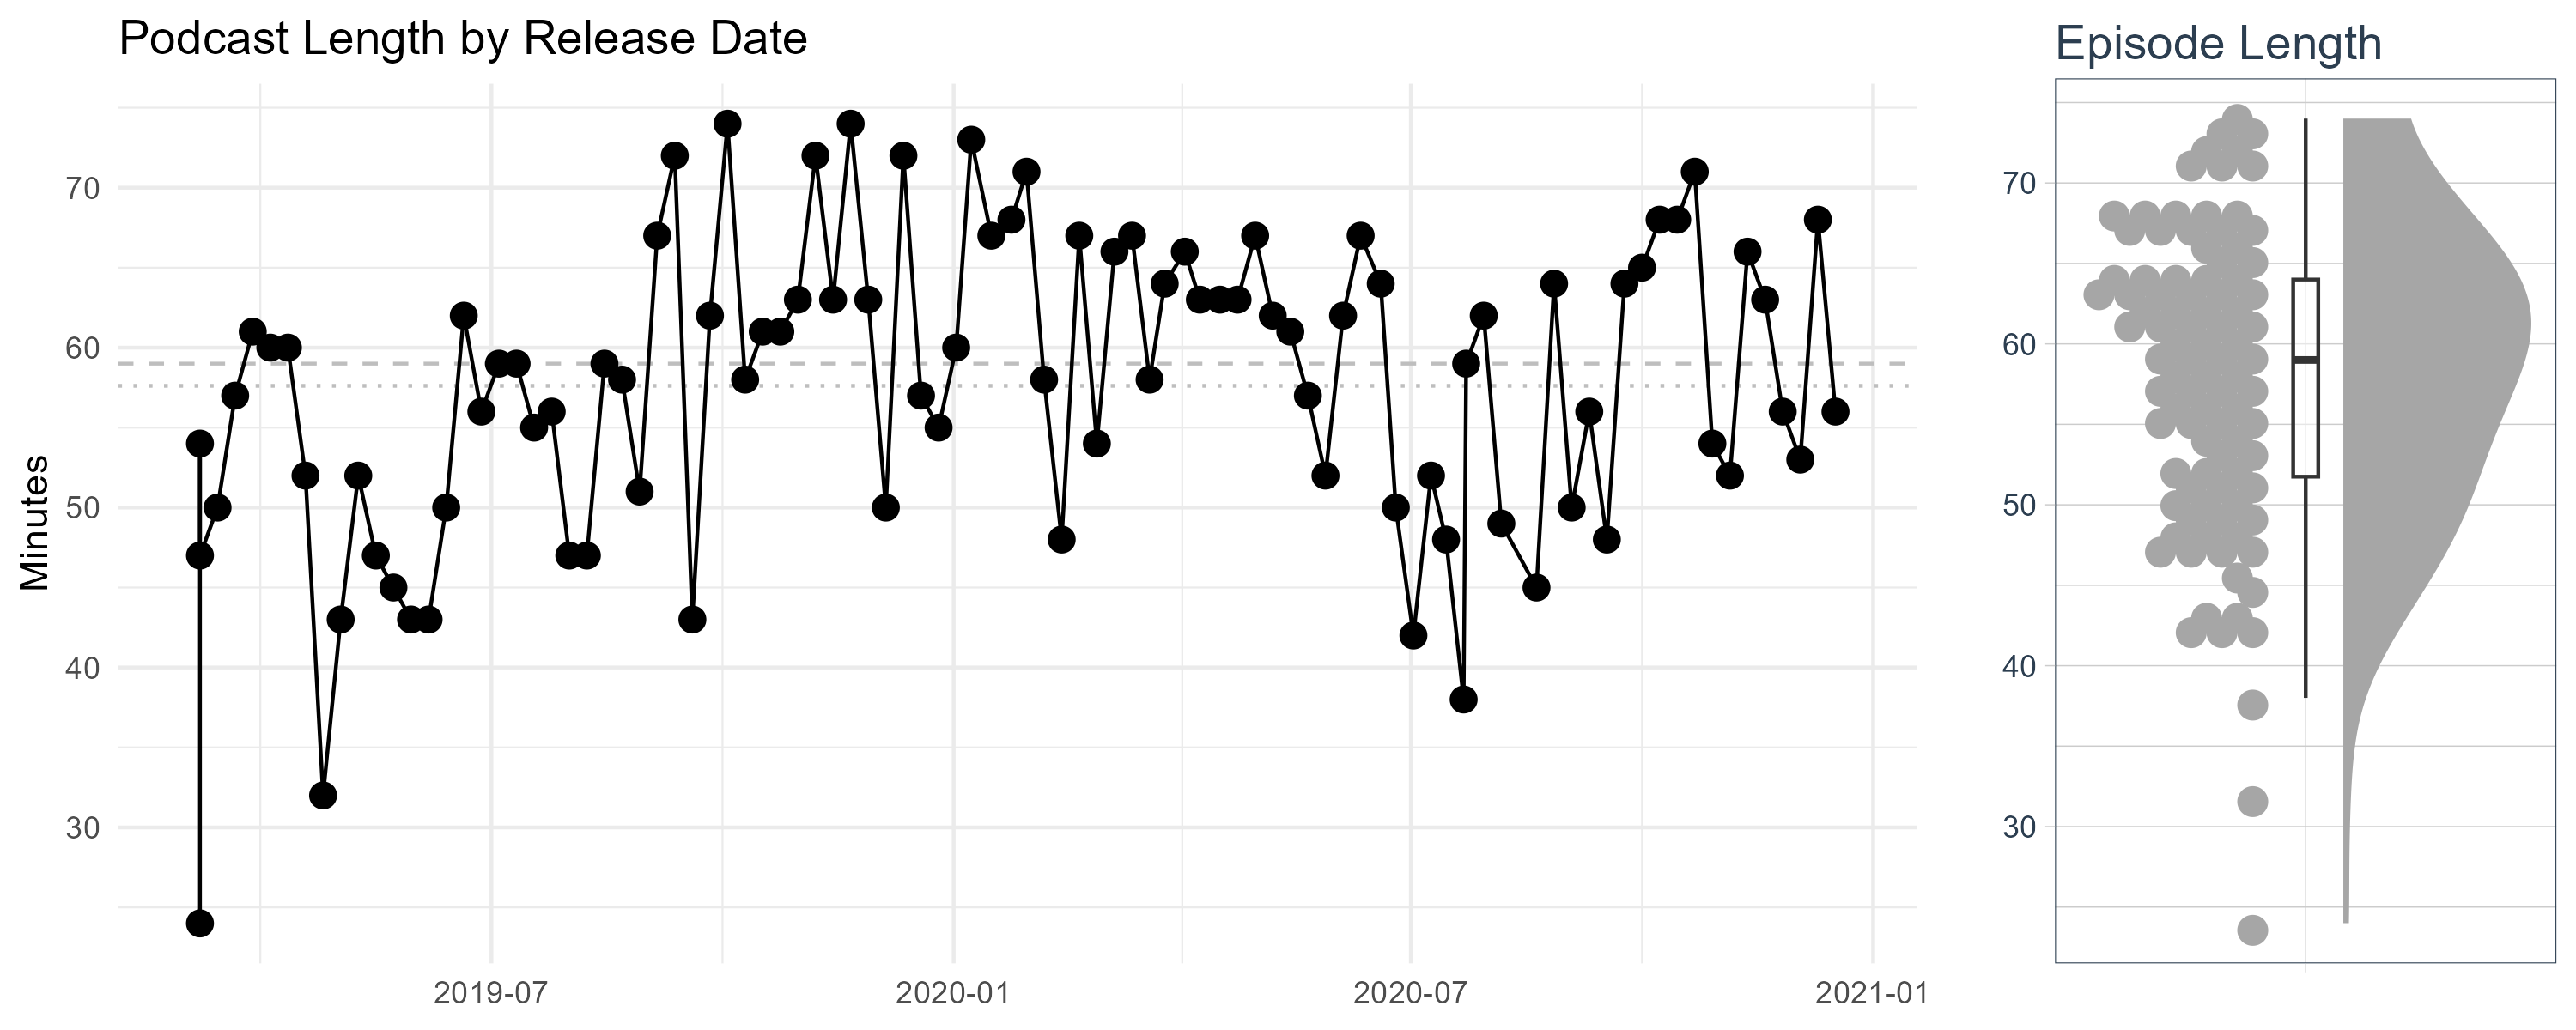
\includegraphics[width=\textwidth]{charts/iskisur_length}

    Over a period of 21 months, there is 5531 minutes of \emph{quality} content, or 3.8 days of continuous
    listening.

    Median length is 59 minutes, but never surpassing 75 minutes.

\end{frame}

\begin{frame}
    \frametitle{Podcast on Storytel: High Ratings}
    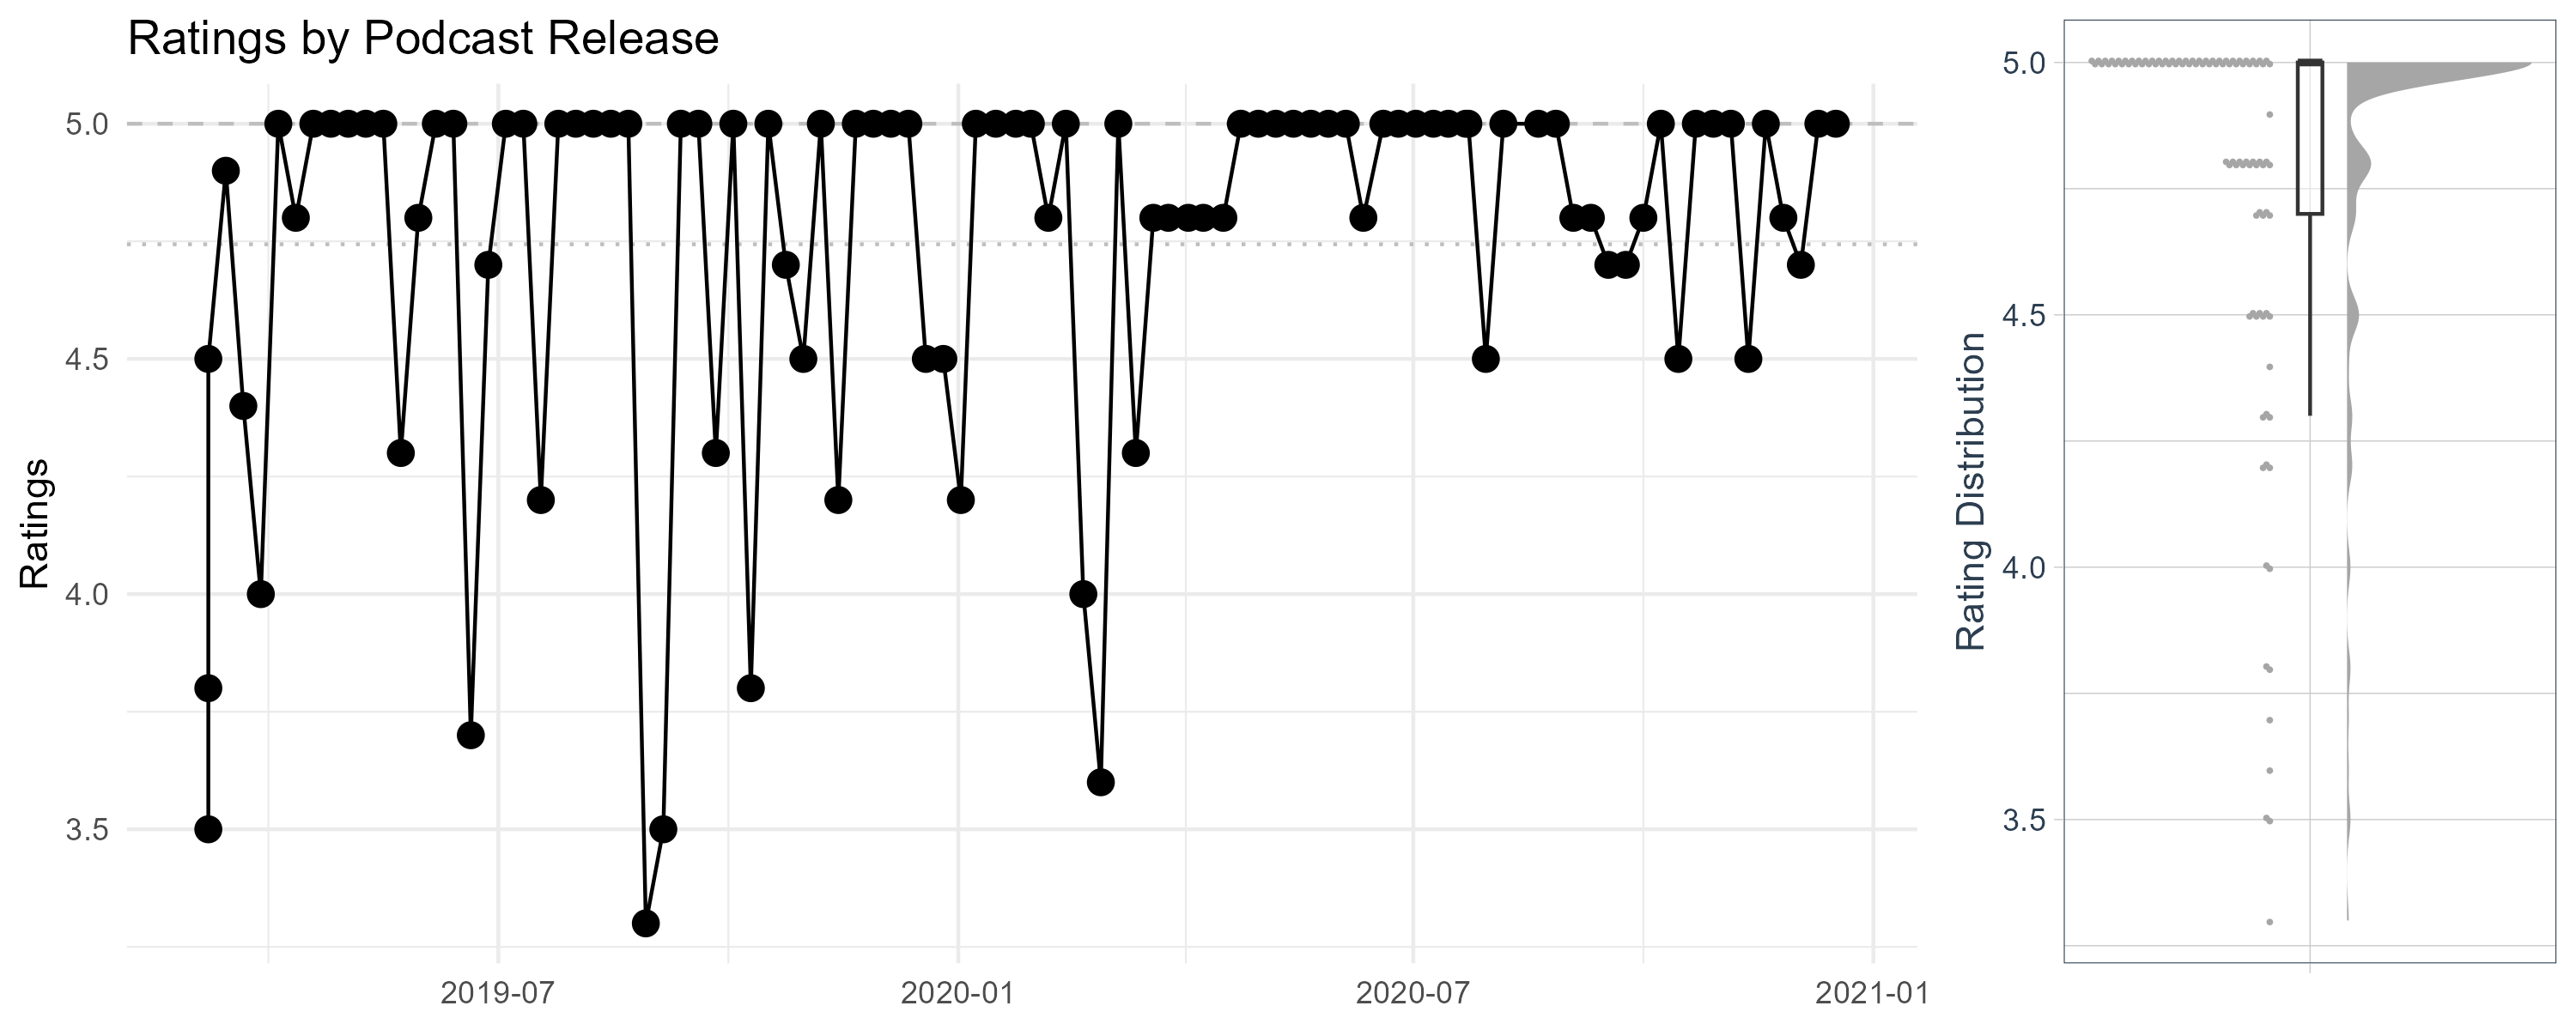
\includegraphics[width=\textwidth]{charts/iskisur_ratings}
    \begin{itemize}
        \item Average rating: 4.74 out of 5
        \item 54 episodes with a perfect 5.0 score (56\% of total)
        \item Only 4 episodes with a rating below 4.0 (worst case 3.3)
    \end{itemize}
\end{frame}

\begin{frame}
    \frametitle{Podcast on Storytel: Low Reviews}
    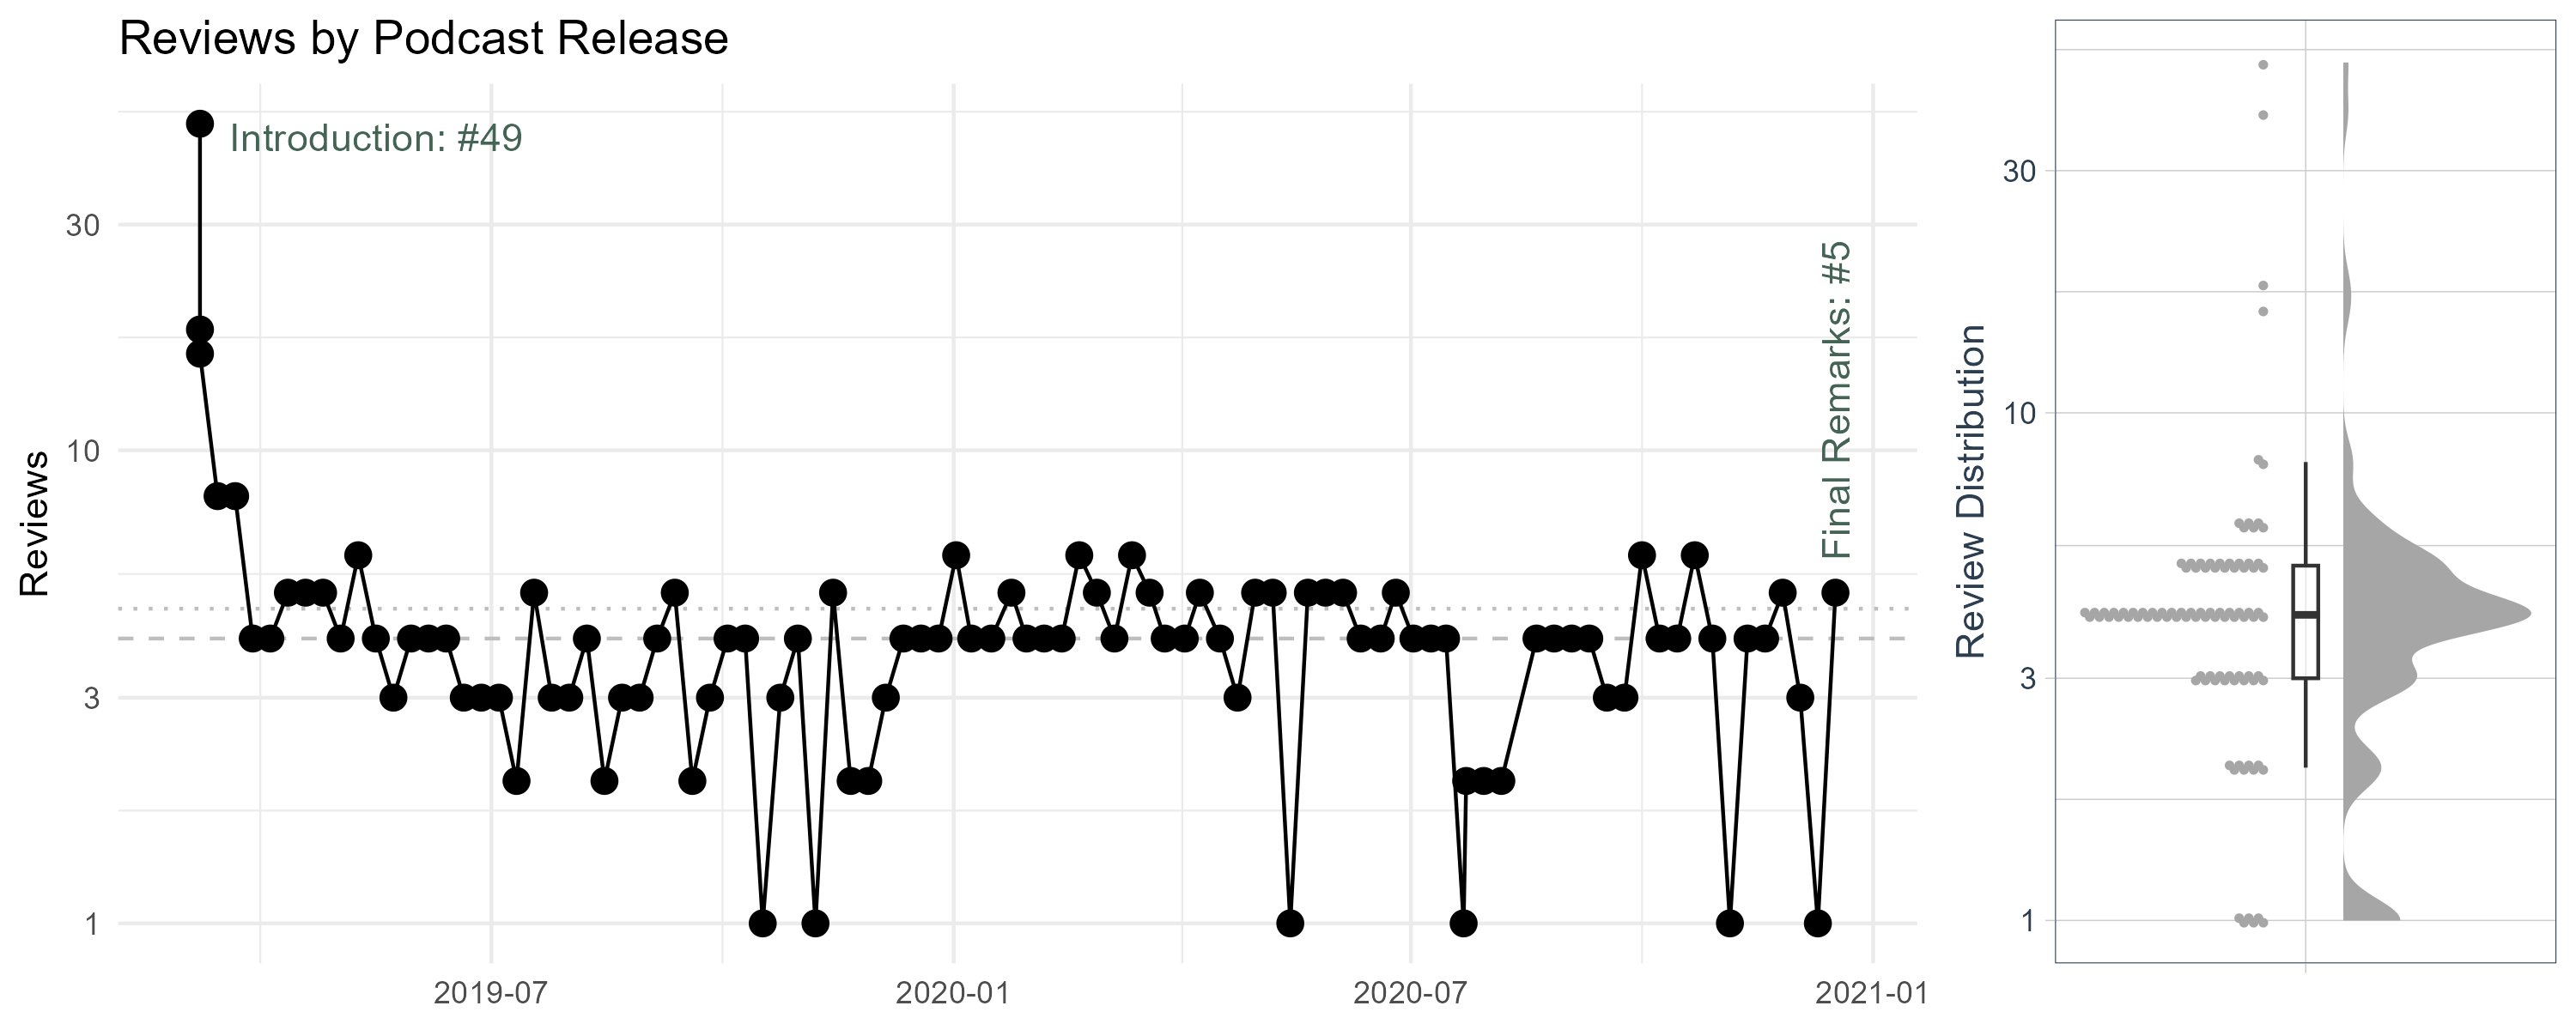
\includegraphics[width=\textwidth]{charts/iskisur_reviews}

    \begin{itemize}
        \item Number of reviews: 444 total (25,627 for the audiobooks)
        \item At least one active fan throughout the period
        \item Four regular fans who consistently provided review
    \end{itemize}

    %Please note that while the high ratings may seem impressive, we humbly acknowledge that they might not be
    %entirely trustworthy. The number of reviews for the podcast, 444 in total, pales in comparison to the 25,
    %627 reviews received for the audio books. Nevertheless, we are grateful for the 49 reviews received for
    %the inaugural introduction episode, and we appreciate the dedication of at least one active fan
    %throughout the podcast's duration. Additionally, we extend our heartfelt thanks to the four regular fans
    %who consistently supported us by providing reviews.

\end{frame}

\begin{frame}
    \frametitle{Podcast Platform Comparison}

    \begin{table}[]
        \begin{tabular}{l|rr|rr|rrr|r}
            & \rotatebox{90}{Episodes} & \rotatebox{90}{Books} &
            \rotatebox{90}{Total Running Time (hours)} & \rotatebox{90}{Average Length (min)} &
            \rotatebox{90}{Median Days to Next}
            & \rotatebox{90}{Average Days to Next}  & \rotatebox{90}{Max Days to Next}  &
            \rotatebox{90}{Months Active} \\
            \midrule
            Alvarpi\dh & 46  & 6  & 37.2  & 48.50 & 7 & 13.69 & 161 & 20.3  \\
            Storytel   & 96  & 47 & 92.2  & 57.61 & 7 & 6.85  & 14  & 21.4  \\
            \midrule
            & 142 &    & 129.4 &       &   &       &     & 45.8*
        \end{tabular}
    \end{table}

    \vfill
    \footnotesize{*4.1 months hiatus between Alvarpi\dh{} and Storytel}
\end{frame}

